Based on the transmitting frequency range of the SDR the size and type of two antennas will be determined.
They will be etched on printed circuit boards that will be submerged in the liquid.
On the end of those antenna PCBs there are sockets for attaching cables that run from the SDR to the antennas.
No other circuit components will be necessary.

\begin{center}
    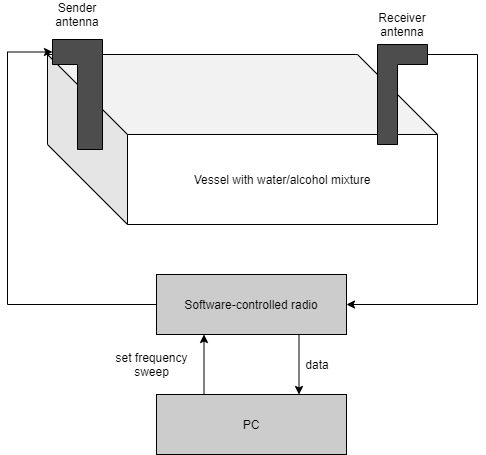
\includegraphics[scale=0.25]{sensor_system.png}
\end{center}

A program will be made to transmit radio waves with a frequency sweep.
Based on the magnitude and phase shift of the received radio waves the program should be able to calculate the dielectric constant of the liquid.
The formula of a mixture's dielectric constant is
\begin{align}
    \epsilon_m = \epsilon_2 + \left( \epsilon_1 - \epsilon_2 \right) \sigma_1
\end{align}
where $\epsilon_m$ is the mixture's dielectric constant, $\epsilon_1$ and $\epsilon_2$ are the dielectric constants of the mixed elements and $\sigma_1$ is the concentration of the first solvent in the mixture.
This formula can be rearranged to get that
\begin{align}
    \sigma_1 = \frac{\epsilon_2 - \epsilon_m}{\epsilon_2 - \epsilon_1}
\end{align}
If we know the dielectric constant of the mixture, and the separate constants for pure water and pure ethyl alcohol, we can determine the ratio of water-to-alcohol in the mixture.